\documentclass[aspectratio=169]{beamer}
\usepackage{animate}
\usepackage{xcolor}
\usepackage[absolute,overlay]{textpos}
\usepackage[textfont={scriptsize}]{caption}
\usepackage{booktabs}

\usetheme{Boadilla}

\newcommand\email[1]{\def\insertemail{#1}}
\providecommand\insertemail{\texttt{alefilot@auth.gr}}
% No slide numbering

\setbeamertemplate{footline}
{
\leavevmode%
\hbox{%
\begin{beamercolorbox}[wd=.3\paperwidth,ht=2.25ex,dp=1ex,center]{author in head/foot}%
\usebeamerfont{author in head/foot}\insertshortauthor~~(\insertshortinstitute)
\end{beamercolorbox}%
\begin{beamercolorbox}[wd=.5\paperwidth,ht=2.25ex,dp=1ex,center]{title in head/foot}%
\usebeamerfont{title in head/foot}\insertshorttitle
\end{beamercolorbox}%
%\begin{beamercolorbox}[wd=.2\paperwidth,ht=2.25ex,dp=1ex,right]{date in head/foot}%
%\usebeamerfont{date in head/foot}\insertshortdate{}\hspace*{2em}
%%#turning the next line into a comment, erases the frame numbers
%%\insertframenumber{} / \inserttotalframenumber\hspace*{2ex}
%\end{beamercolorbox}}%
\begin{beamercolorbox}[wd=.2\paperwidth,ht=2.25ex,dp=1ex,center]{date in head/foot}%
\usebeamerfont{date in head/foot}\insertemail{}
%#turning the next line into a comment, erases the frame numbers
%\insertframenumber{} / \inserttotalframenumber\hspace*{2ex}
\end{beamercolorbox}}%
\vskip0pt%
}

%remove navigation symbols
\setbeamertemplate{navigation symbols}{}


\definecolor{my_red}{rgb}{0.894,0.102,0.110}
\definecolor{my_blue}{rgb}{0.215,0.494,0.721}




\title{FSM: Correspondenceless scan-matching of panoramic 2D range scans}
%\subtitle{}
\author[Alexandros Filotheou et al.]{\small Alexandros Filotheou, Antonis Dimitriou \& Georgios Sergiadis}
\institute[AUTh GR]{Aristotelian University of Thessaloniki (AUTh), Greece}
\date{}

\titlegraphic{
  \includegraphics[width=1cm]{./figures/auth_logo}\hspace*{-11.75cm}\vspace{-2cm}~%
}

\newlength\imageheight
\newlength\imagewidth

\begin{document}

\begin{frame}[noframenumbering]
\titlepage
\end{frame}


\begin{frame}[noframenumbering]{Summary}

\begin{overlayarea}{\textwidth}{3cm}
\leavevmode
  \begin{itemize}
    \item It is possible to match 2D range scans \textbf{without establishing correspondences}\\
          \textit{if their FOV is} $2\pi$ rad
    \item<2|only@2> Leads to increased accuracy \& robustness in the face of sensor noise
    \item<3|only@3> Leads to increased accuracy \& robustness in the face of sensor noise, and fewer parameters needed to be set
  \end{itemize}

\end{overlayarea}
\end{frame}


\begin{frame}[noframenumbering]{Why dispense with correspondences?}

\definecolor{r}{RGB}{255 69 0}
\definecolor{b}{RGB}{51 102 153}

  \begin{figure}\vspace{1cm}
    \animategraphics[height=135pt,width=240pt,autoplay,loop]{5}{./figures/02/pic}{0}{50}
    \caption{Matching with correspondences in ideal conditions. Sensor noise:
             $\mathcal{N}(0,0)$ [m,m$^2$]. Final estimation errors: $0.0023$ m, $0.006$
             rad. Adapted from
             \url{https://nbviewer.org/github/niosus/notebooks/blob/master/icp.ipynb},
             courtesy of Igor Bogoslavskyi}
    \begin{textblock}{5}(3.4,3.2)
      \scriptsize Euclidean Space $|$ \textcolor{r}{$\mathcal{S}_{\text{ref}}$},\textcolor{b}{$\mathcal{S}_{\text{sens}}$}
    \end{textblock}
    \begin{textblock}{4}(8.4,3.2)
      \scriptsize Correspondences' space
    \end{textblock}
  \end{figure}

\end{frame}

\begin{frame}[noframenumbering]{Why dispense with correspondences?}

\begin{overlayarea}{\textwidth}{3cm}
\leavevmode
  \begin{itemize}
    \item Sensor noise
  \end{itemize}

\end{overlayarea}

\end{frame}


\begin{frame}[noframenumbering]{Why dispense with correspondences?}

  \begin{figure}\vspace{1cm}
    \animategraphics[height=135pt,width=240pt,autoplay,loop]{5}{./figures/03/pic}{0}{50}
    \caption{Matching with correspondences in real conditions. Sensor noise:
             $\mathcal{N}(0, 0.10^2)$. Final estimation errors:
             $0.035$ m, $0.011$ rad. Adapted from
             \url{https://nbviewer.org/github/niosus/notebooks/blob/master/icp.ipynb},
              courtesy of Igor Bogoslavskyi}
    \begin{textblock}{3}(4.4,3.2)
      \scriptsize Euclidean Space
    \end{textblock}
    \begin{textblock}{4}(8.4,3.2)
      \scriptsize Correspondences' space
    \end{textblock}
  \end{figure}

\end{frame}


\begin{frame}[noframenumbering]{Why dispense with correspondences?}

\begin{overlayarea}{\textwidth}{3cm}
\leavevmode
  \begin{itemize}
    \item Sensor noise
    \item Void correspondences (outliers)
  \end{itemize}

\end{overlayarea}

\end{frame}


\begin{frame}[noframenumbering]{Why dispense with correspondences?}

  Ultimately:
  \begin{itemize}
    \item Due to sensor noise (higher as sensor cost decreases)
    \item Void (and false) correspondences' rejection is based on offline- and user-set parameters
  \end{itemize}

  \vfill
  {\tiny
  More details: \\
  Filotheou, A. et al. ``Passive Global Localisation of Mobile Robot via 2D
  Fourier-Mellin Invariant Matching". \\ \vspace{-0.25cm}
  In \textit{Journal of Intelligent \& Robotic Systems} 104 (2022). \url{https://doi.org/10.1007/s10846-021-01535-7}}

\end{frame}


\begin{frame}[noframenumbering]{Why dispense with correspondences?}

  \begin{figure}\vspace{1cm}
    \animategraphics[height=135pt,width=180pt,autoplay,loop]{5}{./figures/06/pic}{0}{19}
    \caption{Matching without correspondences in real conditions, with
             outliers/void correspondences. Sensor noise:
             $\mathcal{N}(0, 0.10^2)$ [m,m$^2$]. Final estimation errors: $0.018$ m,
             $0.0008$ rad}
  \end{figure}

\end{frame}


\begin{frame}[noframenumbering]{The Fourier Scan Matcher (FSM)}

  \begin{itemize}
    \item Operates on panoramic scans ($\text{FOV} = 2\pi$ rad)
    \item Does not deal in correspondences between inputs
    \item Requires minimal (if any) tuning
  \end{itemize}

\end{frame}

\begin{frame}[noframenumbering]{The Fourier Scan Matcher (FSM)}

\definecolor{r}{RGB}{255 69 0}
\definecolor{b}{RGB}{51 102 153}

  \begin{center}
    Operating principle: \\
    Scan--to--map-scan matching \\
  \end{center}

  \begin{itemize}
    \item \textcolor{r}{$\mathcal{S}_{\text{ref}}$} projected to 2D plane $\Rightarrow$ map $\bm{M}$
    \item \textcolor{b}{$\mathcal{S}_{\text{sens}}$} matched against scans derived within $\bm{M}$ (so-called \textit{map-scans} $\mathcal{S}^{\bm{M}}$)
  \end{itemize}

\end{frame}


\begin{frame}[noframenumbering]

  \frametitle{Correspondenceless solution to orientation estimation}


  \vspace{0.1cm}
  \setbeamertemplate{itemize items}[circle]
  \begin{itemize}
    \item Via 1D Phase-only Matched Filtering (error $\leq \dfrac{\text{angle increment}}{2}$)
  \end{itemize}
  \vspace{-0.25cm}

  % https://tex.stackexchange.com/questions/240243/getting-gif-and-or-moving-images-into-a-latex-presentation
  \begin{center}
    \animategraphics[height=200pt,width=267pt,autoplay,loop,trim=0 50 0 50,keepaspectratio]{2}{./figures/rotation/rotation_only_fig}{2}{4}
  \end{center}

\end{frame}


\begin{frame}[noframenumbering]

  \frametitle{Correspondenceless solution to translation estimation}

  \vspace{0.1cm}
  \setbeamertemplate{itemize items}[circle]
  \begin{itemize}
    \item Continuous space solution; feedback of DFT difference between scans
  \end{itemize}
  \vspace{-0.5cm}

  % https://tex.stackexchange.com/questions/240243/getting-gif-and-or-moving-images-into-a-latex-presentation
  \begin{center}
    \animategraphics[height=170pt,width=226.67pt,autoplay,loop]{2}{./figures/translation/translation_only_fig}{2}{8}
  \end{center}

  \vfill
  {\tiny
  More details: \\
  Filotheou, A. ``Correspondenceless scan-to-map-scan matching of homoriented 2D scans for mobile robot localisation". \\\vspace{-0.25cm}
  In \textit{Robotics and Autonomous Systems} 149 (2022). \url{https://doi.org/10.1016/j.robot.2021.103957}}

\end{frame}


\begin{frame}[noframenumbering]

  \frametitle{FSM alignment progress and properties}

  % https://tex.stackexchange.com/questions/240243/getting-gif-and-or-moving-images-into-a-latex-presentation
  \begin{center}\vspace{-0.6cm}
    \animategraphics[height=240pt,width=320pt,autoplay,keepaspectratio,trim=0 100 0 0]{3}{./figures/translation_and_rotation/all_fig}{2}{11}
  \end{center}

\end{frame}

\input{slides/10/10_1.tex}
\begin{frame}[noframenumbering]

  \frametitle{FSM alignment progress and properties}


  % https://tex.stackexchange.com/questions/240243/getting-gif-and-or-moving-images-into-a-latex-presentation
  \begin{center}
    \includegraphics[height=240pt,width=320pt]{./figures/translation_and_rotation/all_fig13.png}
  \end{center}

\end{frame}

\begin{frame}[noframenumbering]

  \frametitle{FSM alignment progress and properties}


  % https://tex.stackexchange.com/questions/240243/getting-gif-and-or-moving-images-into-a-latex-presentation
  \begin{center}
    \includegraphics[height=200pt,width=267pt]{./figures/translation_and_rotation/all_fig14.png}
  \end{center}

\end{frame}


\begin{frame}[noframenumbering]{Laser odometry comparison}

  Sensor: YDLIDAR TG30

  \begin{table}[h]\centering \vspace{0.5cm}
    \begin{tabular}{rc}
      Range $d$ [mm]   & Mean error [mm]    \\ \toprule
      $50$-$5000$      & $\leq \pm 60$      \\
      $5000$-$20000$   & $\leq \pm 40$      \\
      $20000$-$30000$  & $\leq \pm 100$     \\ \bottomrule
    \end{tabular}
    \caption{\scriptsize Sensor noise properties (knowledge of distribution N/A).
             Source: \url{www.ydlidar.com/Public/upload/files/2022-06-21/YDLIDAR\%20TG30\%20Data\%20Sheet\%20V1.4(211230).pdf}}
  \end{table}

\end{frame}

\begin{frame}[noframenumbering]{Laser odometry comparison}

  \begin{figure}
    \input{./figures/11/laser_odometry_plicp_fsm.tex}
  \end{figure}

\end{frame}

\begin{frame}[noframenumbering]{Laser odometry comparison}

  \begin{figure}
    \input{./figures/11/laser_odometry_ndt_fsm.tex}
  \end{figure}

\end{frame}

\begin{frame}[noframenumbering]{Laser odometry comparison}

  \begin{figure}
    \definecolor{plicp}{rgb}{0.00000   0.44700   0.74100}
\definecolor{ndt}{rgb}{0.85000   0.32500   0.09800}
\definecolor{fgi}{rgb}{0.9290 0.6940 0.1250}
\definecolor{fvg}{rgb}{0.4940 0.1840 0.5560}
\definecolor{fmt}{rgb}{1.00000   0.00000   1.00000}
\definecolor{gg}{RGB}{156 156 156}

% GNUPLOT: LaTeX picture with Postscript
\begingroup
  \makeatletter
  \providecommand\color[2][]{%
    \GenericError{(gnuplot) \space\space\space\@spaces}{%
      Package color not loaded in conjunction with
      terminal option `colourtext'%
    }{See the gnuplot documentation for explanation.%
    }{Either use 'blacktext' in gnuplot or load the package
      color.sty in LaTeX.}%
    \renewcommand\color[2][]{}%
  }%
  \providecommand\includegraphics[2][]{%
    \GenericError{(gnuplot) \space\space\space\@spaces}{%
      Package graphicx or graphics not loaded%
    }{See the gnuplot documentation for explanation.%
    }{The gnuplot epslatex terminal needs graphicx.sty or graphics.sty.}%
    \renewcommand\includegraphics[2][]{}%
  }%
  \providecommand\rotatebox[2]{#2}%
  \@ifundefined{ifGPcolor}{%
    \newif\ifGPcolor
    \GPcolorfalse
  }{}%
  \@ifundefined{ifGPblacktext}{%
    \newif\ifGPblacktext
    \GPblacktexttrue
  }{}%
  % define a \g@addto@macro without @ in the name:
  \let\gplgaddtomacro\g@addto@macro
  % define empty templates for all commands taking text:
  \gdef\gplfronttext{}%
  \gdef\gplfronttext{}%
  \makeatother
  \ifGPblacktext
    % no textcolor at all
    \def\colorrgb#1{}%
    \def\colorgray#1{}%
  \else
    % gray or color?
    \ifGPcolor
      \def\colorrgb#1{\color[rgb]{#1}}%
      \def\colorgray#1{\color[gray]{#1}}%
      \expandafter\def\csname LTw\endcsname{\color{white}}%
      \expandafter\def\csname LTb\endcsname{\color{black}}%
      \expandafter\def\csname LTa\endcsname{\color{black}}%
      \expandafter\def\csname LT0\endcsname{\color[rgb]{1,0,0}}%
      \expandafter\def\csname LT1\endcsname{\color[rgb]{0,1,0}}%
      \expandafter\def\csname LT2\endcsname{\color[rgb]{0,0,1}}%
      \expandafter\def\csname LT3\endcsname{\color[rgb]{1,0,1}}%
      \expandafter\def\csname LT4\endcsname{\color[rgb]{0,1,1}}%
      \expandafter\def\csname LT5\endcsname{\color[rgb]{1,1,0}}%
      \expandafter\def\csname LT6\endcsname{\color[rgb]{0,0,0}}%
      \expandafter\def\csname LT7\endcsname{\color[rgb]{1,0.3,0}}%
      \expandafter\def\csname LT8\endcsname{\color[rgb]{0.5,0.5,0.5}}%
    \else
      % gray
      \def\colorrgb#1{\color{black}}%
      \def\colorgray#1{\color[gray]{#1}}%
      \expandafter\def\csname LTw\endcsname{\color{white}}%
      \expandafter\def\csname LTb\endcsname{\color{black}}%
      \expandafter\def\csname LTa\endcsname{\color{black}}%
      \expandafter\def\csname LT0\endcsname{\color{black}}%
      \expandafter\def\csname LT1\endcsname{\color{black}}%
      \expandafter\def\csname LT2\endcsname{\color{black}}%
      \expandafter\def\csname LT3\endcsname{\color{black}}%
      \expandafter\def\csname LT4\endcsname{\color{black}}%
      \expandafter\def\csname LT5\endcsname{\color{black}}%
      \expandafter\def\csname LT6\endcsname{\color{black}}%
      \expandafter\def\csname LT7\endcsname{\color{black}}%
      \expandafter\def\csname LT8\endcsname{\color{black}}%
    \fi
  \fi
    \setlength{\unitlength}{0.0500bp}%
    \ifx\gptboxheight\undefined%
      \newlength{\gptboxheight}%
      \newlength{\gptboxwidth}%
      \newsavebox{\gptboxtext}%
    \fi%
    \setlength{\fboxrule}{0.5pt}%
    \setlength{\fboxsep}{1pt}%
\begin{picture}(4000.00,4000.00)%
    \gplgaddtomacro\gplfronttext{%
      \put(1200,4000){\makebox(0,0){\strut{}{\color{fgi}{\rule[0.6mm]{0.5cm}{0.5mm}}} \texttt{FastGICP}}}
      \put(2800,4000){\makebox(0,0){\strut{}{\color{fmt}{\rule[0.6mm]{0.5cm}{0.5mm}}} \texttt{FSM}}}
    }%
    \gplgaddtomacro\gplfronttext{%
      \colorrgb{0.15,0.15,0.15}%
      \put(-92,3526){\makebox(0,0)[r]{\strut{}	\tiny $21.0$}}%
      \colorrgb{0.15,0.15,0.15}%
      \put(-92,3065){\makebox(0,0)[r]{\strut{}	\tiny $19.0$}}%
      \colorrgb{0.15,0.15,0.15}%
      \put(-92,2604){\makebox(0,0)[r]{\strut{}	\tiny $17.0$}}%
      \colorrgb{0.15,0.15,0.15}%
      \put(-92,2143){\makebox(0,0)[r]{\strut{}	\tiny $15.0$}}%
      \colorrgb{0.15,0.15,0.15}%
      \put(271,3746){\makebox(0,0){\strut{}	\tiny $12.0$}}%
      \colorrgb{0.15,0.15,0.15}%
      \put(1193,3746){\makebox(0,0){\strut{}	\tiny $16.0$}}%
      \colorrgb{0.15,0.15,0.15}%
      \put(2115,3746){\makebox(0,0){\strut{}	\tiny $20.0$}}%
      \colorrgb{0.15,0.15,0.15}%
      \put(3037,3746){\makebox(0,0){\strut{}	\tiny $24.0$}}%
      \colorrgb{0.15,0.15,0.15}%
      \put(3959,3746){\makebox(0,0){\strut{}	\tiny $28.0$}}%
    }%
    \gplgaddtomacro\gplfronttext{%
    }%
    \gplgaddtomacro\gplfronttext{%
      \colorrgb{0.15,0.15,0.15}%
      \put(-92,1726){\makebox(0,0)[r]{\strut{}	\tiny $21.0$}}%
      \colorrgb{0.15,0.15,0.15}%
      \put(-92,1265){\makebox(0,0)[r]{\strut{}	\tiny $19.0$}}%
      \colorrgb{0.15,0.15,0.15}%
      \put(-92,804){\makebox(0,0)[r]{\strut{}	\tiny $17.0$}}%
      \colorrgb{0.15,0.15,0.15}%
      \put(-92,343){\makebox(0,0)[r]{\strut{}	\tiny $15.0$}}%
      \colorrgb{0.15,0.15,0.15}%
      \put(271,-108){\makebox(0,0){\strut{}	\tiny $12.0$}}%
      \colorrgb{0.15,0.15,0.15}%
      \put(1193,-108){\makebox(0,0){\strut{}	\tiny $16.0$}}%
      \colorrgb{0.15,0.15,0.15}%
      \put(2115,-108){\makebox(0,0){\strut{}	\tiny $20.0$}}%
      \colorrgb{0.15,0.15,0.15}%
      \put(3037,-108){\makebox(0,0){\strut{}	\tiny $24.0$}}%
      \colorrgb{0.15,0.15,0.15}%
      \put(3959,-108){\makebox(0,0){\strut{}	\tiny $28.0$}}%
    }%
    \put(0,0){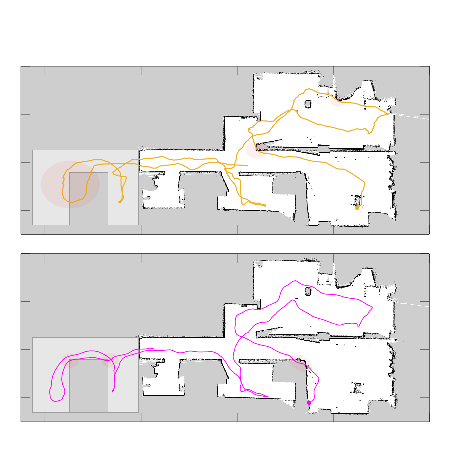
\includegraphics{./figures/11/laser_odometry_fgi_fsm1}}%
    \gplfronttext
  \end{picture}%
\endgroup

  \end{figure}\end{frame}

\input{slides/11/11_4.tex}

\begin{frame}[noframenumbering]{FSM: Correspondenceless scan-matching of panoramic 2D range scans}

\begin{center}
  Thank you for your attention
\end{center}

  \vspace{2cm}

  \begin{itemize}
    \item \scriptsize Presentation available at \url{www.github.com/li9i}
    \item \scriptsize Code available at \url{www.github.com/li9i/fsm}
  \end{itemize}

\end{frame}




\end{document}
